%\documentclass[a4paper, 10pt, conference]{../../templates/IEEEconf/IEEEconf}
\documentclass[10pt, conference, onecolumn]{../../../templates/IEEEtran/IEEEtran}
%\documentclass[10pt, journal]{../../templates/IEEEtran/IEEEtran}

\usepackage{graphicx}
\usepackage{caption} 
\usepackage{subcaption}
\usepackage{hyperref}
\usepackage{listings}
\usepackage{hhline}
\usepackage{float}
\usepackage{amssymb}
\usepackage[autostyle=true]{csquotes}
\usepackage{amsmath}
\usepackage{marvosym}
\usepackage{minted}

\font\subtitlefont=cmr12 at 18pt

\title{First contact: Agents meet Haskell \\ {\huge Simulating epidemics using Functional Reactive Programming} \\ {\large An Agent-Based Approach}}

% IEEEtran journal authors
%\author{Jonathan Thaler, ̃Peer-Olaf Siebers \\ School of Computer Science \\ University of Nottingham%
%\thanks{jonathan.thaler@nottingham.ac.uk}%
%\thanks{peer-olaf.siebers@nottingham.ac.uk}
%}

% IEEEtran conference authors
\author{
	\IEEEauthorblockN{Jonathan Thaler}
	\IEEEauthorblockA{School of Computer Science\\
		University of Nottingham\\
		jonathan.thaler@nottingham.ac.uk}
		
	\and
		
	\IEEEauthorblockN{Thorsten Altenkirch}
	\IEEEauthorblockA{School of Computer Science\\
		University of Nottingham\\
		thorsten.altenkirch@nottingham.ac.uk}

	\and
	
	\IEEEauthorblockN{Peer-Olaf Siebers}
	\IEEEauthorblockA{School of Computer Science\\
		University of Nottingham\\
		peer-olaf.siebers@nottingham.ac.uk}
}

%\IEEEpubid{0000--0000/00\$00.00 ̃\copyright ̃2015 IEEE}

% IEEEconf authors
%\author{
%	Jonathan Thaler \\
%	\email{jonathan.thaler@nottingham.ac.uk} \\
%	\begin{affiliation}
%		School of Computer Science, University of Nottingham
%	\end{affiliation} \\
%	\and 
%	Peer-Olaf Siebers \\
%	\email{peer-olaf.siebers@nottingham.ac.uk} \\
%	\begin{affiliation}
%		School of Computer Science, University of Nottingham
%	\end{affiliation} 
%	\and 
%	Thorsten Altenkirch \\
%	\email{thorsten.altenkirch@nottingham.ac.uk} \\
%	\begin{affiliation}
%		School of Computer Science, University of Nottingham
%	\end{affiliation} 
%}

\begin{document}
\maketitle 

\begin{abstract}
TODO: cite my own 1st paper from SSC2017: add it to citations

TODO: refine it: start with simulating epidemics and then go into ABS

Agent-Based Simulation (ABS) is a methodology in which a system is simulated in a bottom-up approach by modelling the micro interactions of its constituting parts, called agents, out of which the global macro system behaviour emerges. So far, the Haskell community hasn't been much in contact with the community of ABS due to the latter's primary focus on the object-oriented programming paradigm. This paper tries to bridge the gap between those two communities by introducing the Haskell community to the concepts of ABS. We do this by deriving an agent-based implementation for the simple SIR model from epidemiology. In our approach we leverage the basic concepts of ABS with functional reactive programming from Yampa which results in a surprisingly fresh, powerful and convenient EDSL for formulating ABS in Haskell.
\end{abstract}

\begin{IEEEkeywords}
Functional Reactive Programming, Agent-Based Simulation
\end{IEEEkeywords}

\section{Introduction}
There exists a large number of simulation packages which allow the convenient creation of System Dynamics simulations by straight-forward visual diagram creation. One simply creates stocks and flows, connects them, specifies the flow-rates and initial parameters and then runs the model. An example for such a visual diagram creation in the simulation package AnyLogic can be seen in Figure \ref{fig:sir_stockflow_diagram}.

\begin{figure}
	\centering
	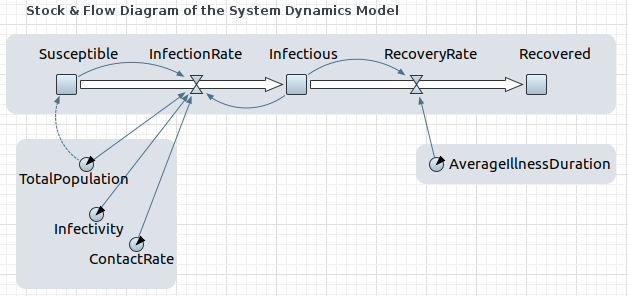
\includegraphics[width=.5\textwidth, angle=0]{./fig/SIR_SD_STOCKFLOW_DIAGRAMM.png}
	\caption{Visual System Dynamics Diagram of the SIR model in AnyLogic Personal Learning Edition 8.3.1.}
	\label{fig:sir_stockflow_diagram}
\end{figure}

Still, implementing System Dynamics directly in code is not as straight forward and involves numerical integration which can be quite tricky to get right. Thus, the aim of this paper is to look into how System Dynamics models can be implemented in code correctly without the use of a simulation package. We use the well known SIR model \cite{kermack_contribution_1927} from epidemiology to demonstrate our approach.

Our language of choice is Haskell because it emphasises a declarative programming style in which one describes \textit{what} instead of \textit{how} to compute. Further it allows to rule out interference with non-deterministic influences or side-effects already at compile-time. This is of fundamental importance for System Dynamics because it behaves completely deterministic and involves no stochastics or non-determinism whatsoever. Also, we make use of Functional Reactive Programming which allows to express continuous-time systems in a functional way. 

We show that by this approach we can arrive at correct-by-construction implementations of System Dynamic models. This means that the correctness of the code is obvious because we have closed the gap between the model specification and its implementation. Thus, the contribution of the paper is the demonstration of how to implement correct-by-construction System Dynamics simulations using Haskell and Functional Reactive Programming.

\section{Defining Agent-Based Simulation}
\label{sec:defining_abs}

Agent-Based Simulation (ABS) is a methodology to model and simulate a system where the global behaviour may be unknown but the behaviour and interactions of the parts making up the system is of knowledge. Those parts, called agents, are modelled and simulated out of which then the aggregate global behaviour of the whole system emerges. So the central aspect of ABS is the concept of an agent which can be understood as a metaphor for a pro-active unit, situated in an environment, able to spawn new agents and interacting with other agents in some neighbourhood by exchange of messages. 
We informally assume the following about our agents \cite{siebers_introduction_2008}, \cite{wooldridge_introduction_2009}, \cite{siebers_discrete-event_2010}, \cite{dawson_opening_2014}, \cite{macal_everything_2016}:

\begin{itemize}
	\item They are uniquely addressable entities with some internal state over which they have full, exclusive control.
	\item They are pro-active which means they can initiate actions on their own e.g. change their internal state, send messages, create new agents, terminate themselves.
	\item They are situated in an environment and can interact with it.
	\item They can interact with other agents which are situated in the same environment by means of messaging.
\end{itemize} 

\begin{comment}
Epstein \cite{epstein_generative_2012} identifies ABS to be especially applicable for analysing \textit{"spatially distributed systems of heterogeneous autonomous actors with bounded information and computing capacity"}. %Thus in the line of the established simulation methodologies (see Table \ref{tab:simulation_types}), ABS is the most powerful one as listed in :
It exhibits the following properties:

\begin{itemize}
	\item Linearity \& Non-Linearity - actions of agents can lead to non-linear behaviour of the system.
	\item Time - agents act over time which is also the source of their pro-activity.
	\item States - agents encapsulate some state which can be accessed and changed during the simulation.
	\item Feedback-Loops - because agents act continuously and their actions influence each other and themselves in subsequent time-steps, feedback-loops are the norm in ABS. 
	\item Heterogeneity - although agents can have same properties like height, sex,... the actual values can vary arbitrarily between agents.
	\item Interactions - agents can be modelled after interactions with an environment or other agents. %, making this a unique feature of ABS, not possible in the other simulation models.
	\item Spatiality \& Networks - agents can be situated within e.g. a spatial (discrete 2D, continuous 3D,...) or complex network environment. % making this also a unique feature of ABS, not possible in the other simulation models.
\end{itemize}
\end{comment}

\begin{comment}
Note that there doesn't exist a commonly agreed technical definition of ABS but the field draws inspiration from the closely related field of Multi-Agent Systems (MAS) \cite{wooldridge_introduction_2009}, \cite{weiss_multiagent_2013}. It is important to understand that MAS and ABS are two different fields where in MAS the focus is much more on technical details, implementing a system of interacting intelligent agents within a highly complex environment with the focus primarily on solving AI problems.
\end{comment}

\section{The SIR Model}
To explain the concepts of ABS and of our functional reactive approach to it, we introduce the SIR model as a motivating example. The SIR model is a a very well studied and understood compartment model from epidemiology which allows to simulate the dynamics of an infectious disease spreading through a population. In this model, people in a population of size $N$ can be in either one of three states \textit{Susceptible}, \textit{Infected} or \textit{Recovered} at a particular time, where it is assumed that initially there is at least one infected person in the population. People interact with each other \textit{on average} with a given rate $\beta$ per time-unit and get infected with a given probability $\gamma$ when interacting with an infected person. When infected, a person recovers \textit{on average} after $\delta$ time-units and is then immune to further infections. An infected person interaction with another infected one is never re-infected, thus interactions amongst infected people is not important in this model. This definition gives rise to three compartments with the transitions as seen in Figure \ref{fig:sir_transitions}.

\begin{figure}
	\centering
	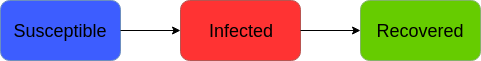
\includegraphics[width=.4\textwidth, angle=0]{./fig/SIR_transitions.png}
	\caption{Transitions in the SIR compartment model.}
	\label{fig:sir_transitions}
\end{figure}

The dynamics of this model over time can be formalized using the following equations:

$\frac{\mathrm d S}{\mathrm d t} = -infectionRate$ \\
$\frac{\mathrm d I}{\mathrm d t} = infectionRate - recoveryRate$ \\
$\frac{\mathrm d R}{\mathrm d t} = recoveryRate$ \\

$infectionRate = \frac{I \beta S \gamma}{N}$ \\
$recoveryRate = \frac{I}{\delta}$ \\

Solving these can be done using the System-Dynamics (SD) approach which solves the equations by integrating over time. In the SD terminology, the intergrals are called \textit{Stocks} and the values over which is integrated over time are called \textit{Flows}.

$S(t) = N + \int_0^t -infectionRate\, \mathrm{d}t$ \\
$I(t) = 1 + \int_0^t infectionRate - recoveryRate\, \mathrm{d}t$ \\
$R(t) = \int_0^t recoveryRate\, \mathrm{d}t$ \\

There exist a huge number of software-packages which allow to conveniently express SD models using a visual approach like in Figure \ref{fig:sir_sd_stockflow_diagramm}.

\begin{figure}
	\centering
	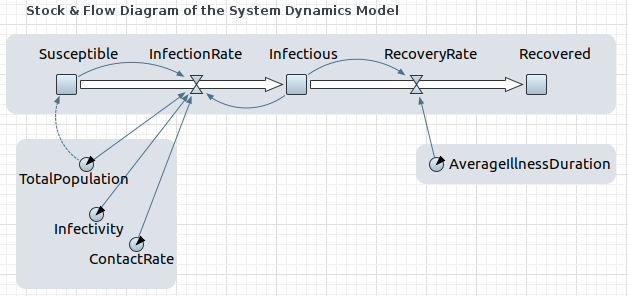
\includegraphics[width=.4\textwidth, angle=0]{./fig/SIR_SD_STOCKFLOW_DIAGRAMM.png}
	\caption{A visual representation of the stocks and flows in the SIR compartment model (Image courtesy of AnyLogic Company).}
	\label{fig:sir_sd_stockflow_diagramm}
\end{figure}

Running the SD simulation over time results in the dynamics as shown in Figure \ref{fig:sir_sd_dynamics_anylogic} with the given variables.

\begin{figure}
	\centering
	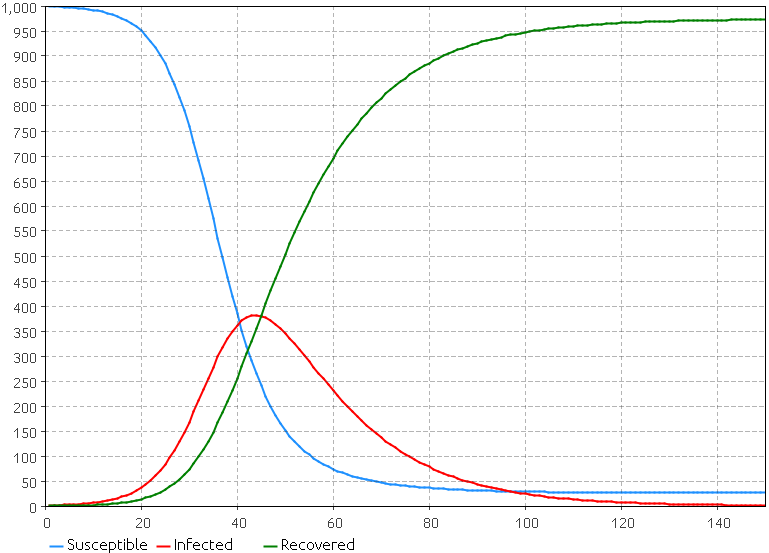
\includegraphics[width=.4\textwidth, angle=0]{./fig/SIR_SD_DYNAMICS_ANYLOGIC.png}
	\caption{Dynamics of the SIR compartment model using the System Dynamics approach generated with the AnyLogic Personal Learning Edition 8.1.0. Population Size $N$ = 1000, contact rate $\beta = 1/5$, infection probability $\gamma = 0.05$, illness duration $\delta = 15$.}
	\label{fig:sir_sd_dynamics_anylogic}
\end{figure}

\subsection{An Agent-Based approach}
The SD approach is inherently Top-Down because the emergent property of the system is formalized in differential equations. The question is if such a top-down behaviour can be emulated using ABS, which is inherently bottom-up. Also the question is if there are fundamental drawbacks and benefits when doing so using ABS. Indeed such questions were asked before and modelling the SD approach of the SIR model is possible using an agent-based approach. It is important to note that SD treats the population completely continuous which results in non-discrete values of stocks e.g. 3.1415 infected persons. Thus the fundamental approach to map the SIR model to an ABS is to discretisize the population and model each person in the population as an invidivual agent. The transition  between the states are no longer happening according to continuous differential equations but due to discrete events caused both by interactions amongst the agents and time-outs. The behaviour can be defined as follows:

\begin{itemize}
	\item Every agent makes on average contact with $\beta$ random other agents per time unit. In ABS we can only contact discrete agents thus we model this by generating a random event on average every $\beta$ time units.
	
	\item An agent does not know the other agents state when making contact with it, thus we need a mechanism in which agents reveal their state in which they are in \textit{at the moment of making contact}. Obviously the already mentioned messaging-mechanism which allows agents to interact is perfectly suited to do this.
	\begin{itemize}
		\item \textit{Susceptible} agent: sends a "Susceptible" message when contacting another agent. There is no need to reply to other incoming messages as making contact with a susceptible agent has no influence on the state of an agent.
		\item \textit{Infected} agent: sends a "Infected" message when contacting another agent. An infected agent now needs to reply to incoming "Susceptible" messages with an "Infected" message to let the susceptible agent know that it has made contact with an infected agent.
		\item \textit{Recovered} agent: does not need to send messages because contacting it or being contacted by it has no influence on the state.
	\end{itemize}
	
	\item Susceptible to Infected: needs to have made contact with an infected agent which happens when it receives an "Infected" message. If this occurs an infection occurs with a probability of $\gamma$. The infection can be calculated by drawing from a uniform random-distribution between 0 and 1 and comparing the value to $\gamma$, if the drawn value $p < \gamma$ then infection occurs. Note that this needs to be done for \textit{every} received "Infected" message.
	
	\item Infected to Recovered: a person recovers \textit{on average} after $\delta$ time unites. This is implemented by drawing the duration from an exponential distribution (TODO: borchschev) with $\lambda = \frac{1}{\delta}$ and making the transition after this duration.
\end{itemize}

We will discuss the implementation of this approach in the following sections and as will be shown FrABS will allow us to express this behaviour very explicitly looking very much like a formal ABS specification of the problem. For now we will give the resulting dynamics in Figure TODO

TODO: how many initially infected agents? one should be enough, at least in my implementation

TODO: 100 vs. 1000 vs. 5.000 agents

TODO: problem in my code: need exponentially occasionally not uniform distributed! => OK, occasionally draws from exponential-distribution
TODO: what differences do the different update strategies make?

\subsection{Blub}
TODO: It should be possible to formally show that spatial SIR and WildFire are the same model. NOTE: they are NOT the same, the fundamental difference is that in the WildFire model only the burning cells initiate the ignition - if we compare this to the SIR, the burning cells would be infected agents and although in the spatial SIR model the infected agents make contact with other agents, so do the susceptible ones which does NOT occur in wildfire

TODO: cite my own work on update-strategies

TODO: can we formally show that the SIR approximates the SD model?

TODO: cite papers which discuss how to approximate a SD model by ABS
- Macal (2010) - To Agent-Based Simulation From System Dynamics 
	-> i am very unhappy with this paper: first it does not give concrete parameters for the SD model so it is impossible to replicate. Also i think it has a systematical error as the infected agents make no contact but this is required as evident from the SD-models infection-rate which also incorporates. TODO: write an email to this guy: why are the infectious not contacting the other agents? this seems to be a systematical error
- Borshchev, Filippov (2004) - From System Dynamics and Discrete Event to Practical Agent Based Modeling: Reasons, Techniques, Tools
	-> its VERY IMPORTANT point is that we need to draw the illness-duration from an exponential-distribution because the illness-duration is proportional to the size of the infected. note: this is wrongly expressed, need to find the correct formulation

		-> my emulation of SD using ABS is really an implementation of the SD model and follows it - they are equivalent
		-> my ABS implementation is the same as / equivalent to the SD emulation
			=> thus if i can show that my SD emulation is equlas to the SD model
			=> AND that the ABS implementation is the same as the SD emulation
			=> THEN the ABS implementation is an SD implementation, and we have shown this in code for the first time in ABS
			


\section*{Acknowledgments}
The authors would like to thank I. Perez, H. Nilsson, J. Greensmith, T. Schwarz and H. Vollbrecht for constructive comments and valuable discussions.

\bibliographystyle{../../../templates/IEEEtran/bibtex/IEEEtran}
\bibliography{../../../../references/phdReferences.bib}

\end{document}